


\documentclass[10pt,journal,compsoc]{IEEEtran}
\providecommand{\PSforPDF}[1]{#1}
\usepackage[english]{babel}
\usepackage{graphicx}


\begin{document}

\title{VLSI Design of CRC-Based Fingerprinting on MIPS8 Architecture}

\author{Georgi Kostadinov, Xinchi Chen, Kaushik Boga, Mojing Liu
\\Department of Electrical and Computer Engineering 
\\McGill University}


\IEEEcompsoctitleabstractindextext{%
\begin{abstract}

Traditional error mitigation techniques such as Error Correcting Code (ECC) and Dual Modular
Redundancy (DMR)  in Lockstep provide error detection at great cost of power, area and performance. In this
paper, we present the implementation and verification of an Execution Fingerprinting Unit using
CRC16 operating on a MIPS8 architecture. Our design provides a 255 times decrease in comparison overhead
compared to DMR Lockstep and 125MHz max operating frequency unpipelined.
\end{abstract}}

\maketitle

\section{Introduction}
\IEEEPARstart{T}{raditional} 
 error mitigation techniques such as Error Correcting Code (ECC) provide limited
error coverage rate at the cost of performance and area overhead. Another solution widely
used in industry,  Dual Modular Redundancy (DMR) in Lockstep, consists of two
redundant cores executing the same application in lockstep and validating the results only if
the comparison passes. However large amount of computational ressource is wasted for comparison
as not to mention the overwhelming complexcity of clock synchronization due to lockstep.

\section{Background}
Fingerprinting first uses Distributed Temporal Redundancy, which allows processors to execute out of sync\cite{DTR}, thus breaking the lockstep. This will create much more freedom in terms of schedulabilty, letting us apply a second technique called Relaxed Dedication which allows the processor to also execute non critical tasks\cite{RD}. 
As the processors are out of sync,however the execution data still needs to be verified through redundant exeuction data. Directly saving the redundant data would not be ressource efficient, hence fingerprinting compresses this block of data into a single word called fingerprint. The compression algorithm can be chosen by the designer and will have different impact in terms of error coverage and detection. 

\section{Implementation }
Fingerprinting can be implemented in three steps. First, the execution data of the processor needs to be extracted and fed into the fingerprinting circuit. Second, this data is compress using CRC16 to generate the fingerprints, which will be explained in details in this section. At last, fingeprints needs to be stored for later comparison for error detection. The implementation of fingerpriting was based on the MIPS8 architecture and a standard cell library provided by Harvey Mudd College\cite{harvey} using Electric VLSI Design System\cite{electric}. The goal of this work is to prove the feasibility of using fingerprinting for error detection Therefore error coverage analysis is not in the scope of this work.

\subsection{Execution Information Extraction}

Only memory write address and data were originally available through the MIPS8 architecture. Fingerprinting additional execution has been proven to improve error dectection coverage and latency\cite{techcon}. Therefore we added to the export list the results of the ALU within the datapath. However, only ALU results that are written to the register file are needed and therefore a control signal composed of \emph{memtoreg} and \emph{regwrite} were used to signal a useful ALU result to be fingerprinted. As the MIPS8 core within this project  cannot ouput a valid ALU result and memory write data, hence an additional multiplexer was added in order to help choosing the right set of signals for the fingerprinting circuit.



\subsection{Compressing the Data: The CRC Fingerprint}

The Cyclic Redundancy Check (CRC) algorithm can be used to compress data for later verification. CRC is a good choice for fingerprinting, because it is a simple and widely used algorithm that was designed with error detection in mind. Although CRC is more ideal for transmission channel error detection, as it can guarantee resilience to burst errors to within a given number of corrupt bits, it can still offer strong error detection for randomly distributed error when compared to other techniques such as Fletcher's Checksum.

A 16-bit wide CRC was chosen, as it offers much stronger error detection characteristics than a lower bit alternative, but is not too large to be considered overkill for a MIPS-8 core. The 0x1755b polynomial was used, since it is a good choice for larger block sizes\cite{Koopman}. A set of logical equations for each output bit were found\cite{Parcrc} and implemented using combinational logic. The produced combinational circuit was linked to a register to store the CRC result after each iteration, as its value is required for the next calculation. 


\subsection{Storing the Fingerprint: Shift Register vs SRAM}
The CRC block generates a fingerprint every 256 memory/ALU operations executed by the MIPS processor. To avoid lockstep execution with a parallel processor, a limited set of these fingerprints are stored in a buffer and read out later for comparison, to detect whether the 256 batch of operations were executed correctly. A buffer size to store 8x16-bit fingerprints was chosen. Since the goal of the project was not memory design, rather to demonstrate the efficacies of fingerprinting, a generic flipflop based shift register circuit was quickly implemented. The generic flipflop takes ph1, ph2, enable and reset as inputs and as a result needed 30 transistors per bit. 

Though the layout was very modular using the standard cell library components, and hence implementation quick, this resulted in a significantly big buffer (needing 3872 transistors) relative to the size of the fingerprinting circuit. This will skew the energy or performance savings primarily proposed. The shift register also suffers from the hold time constraint with a really short contamination delay between two flipflops. So, this implementation would have needed a thorough timing analysis to ensure timing wont fail and is a poor choice of design for a buffer. Hence the shift register was replaced by a FIFO built with SRAM during our optimization phase.

The FIFO features a single read/write per cycle composed of 6T SRAM cells, 2 3-bit counters, row decoder, bitline conditioning and read/write driver logic. Unlike the shift register, the FIFO moves a pointer to the data, instead of moving all the data physically. Two 3-bit counters are used to keep track of read and write pointers to the rows of bits. 3 2:1 multiplexers choose between the two pointers to drive the row decoder depending on whether data is to be read from or written to the SRAM. The row decoder composed of a 2 stage design; 8 3-in NANDs and 8 2-in NORs to drive the word lines. NOR stage makes the row decoder output ph1 qualified to drive the word lines only when ph1 is high. The 16 bitline conditioning blocks sitting on top of the SRAM slices, composed of 2 pmos transistors clocked with ph2b (dynamic logic), precharge the bitlines when ph1 is low, ready for the read/write operation. The read driver is a pair of high skew inverters which detect the voltage on the bitlines and drives the output to the rails or ground. The write driver consists of a series pair of nmos transistors on each bitline. The nmos transistors pull the ‘bit’ line to ground if writeq1 and datas1 are both high and the ‘bitb’ line behaves conversely.  

This implementation needed 1374 transistors laid on a 45 lamda pitch and did not involve moving data around every clock cycle. So, the area and power consumption is much smaller and hence realistic, allowing a more compelling case to be made for the fingerprinting circuit. 


\subsection{The Final Design}
As shown in Fig. 1, the fingerprinting system as a whole includes a multiplexer, a counter, and additional glue logic to integrate the CRC circuit into a fully functional design. The MIPS core serves as the external controller for the fingerprinting system, issuing the appropriate signals whenever new data is ready to be fingerprinted. A multiplexer performs the selection of data to be fingerprinted based on the CPUs signals. A counter is used to count each time new data comes in and it determines the data compression ratio of the fingerprint. When the desired amount of data has been fingerprinted, the counter signals the output buffer block to store the new fingerprint, and it also signals the CRC block to start computation for a new block. The CRC block needs to be able to handle data coming in at the same time as the counter's control signal, so additional logic was required to handle such a scenario. Figure 2 shows the layout of our circuit using SRAM. 

\begin{figure}[h!]
  \centering

      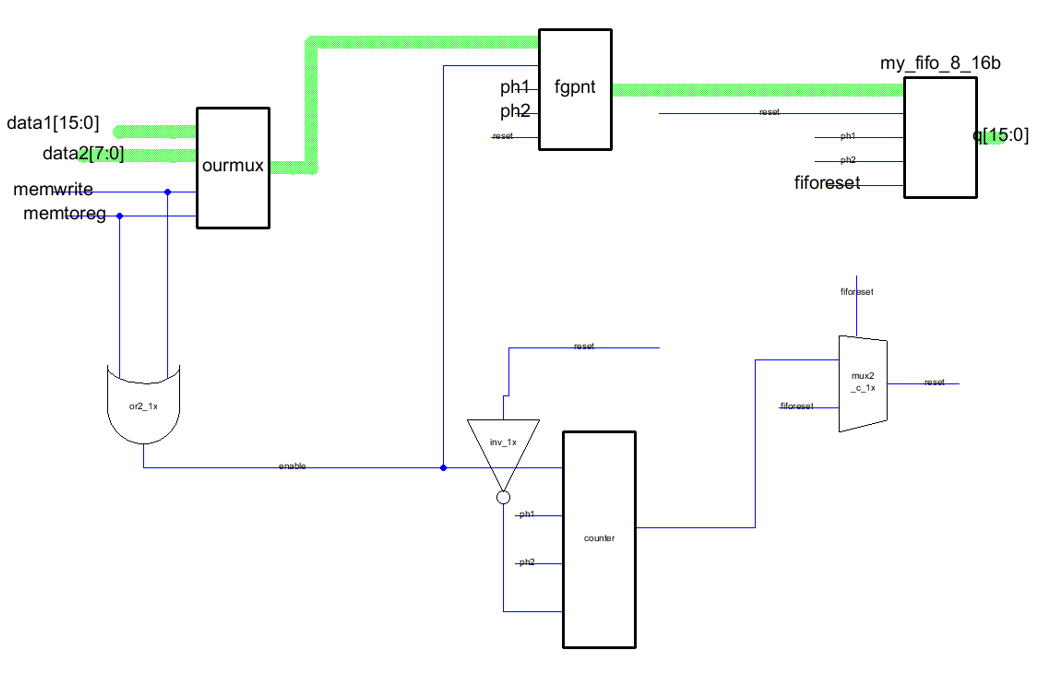
\includegraphics[width=0.5\textwidth]{schematic}
  \caption{Schematic of the fingerprinting circuit with ALU and Memory fingerprinting using a shift register}
\end{figure}
\begin{figure}[h!]
  \centering

      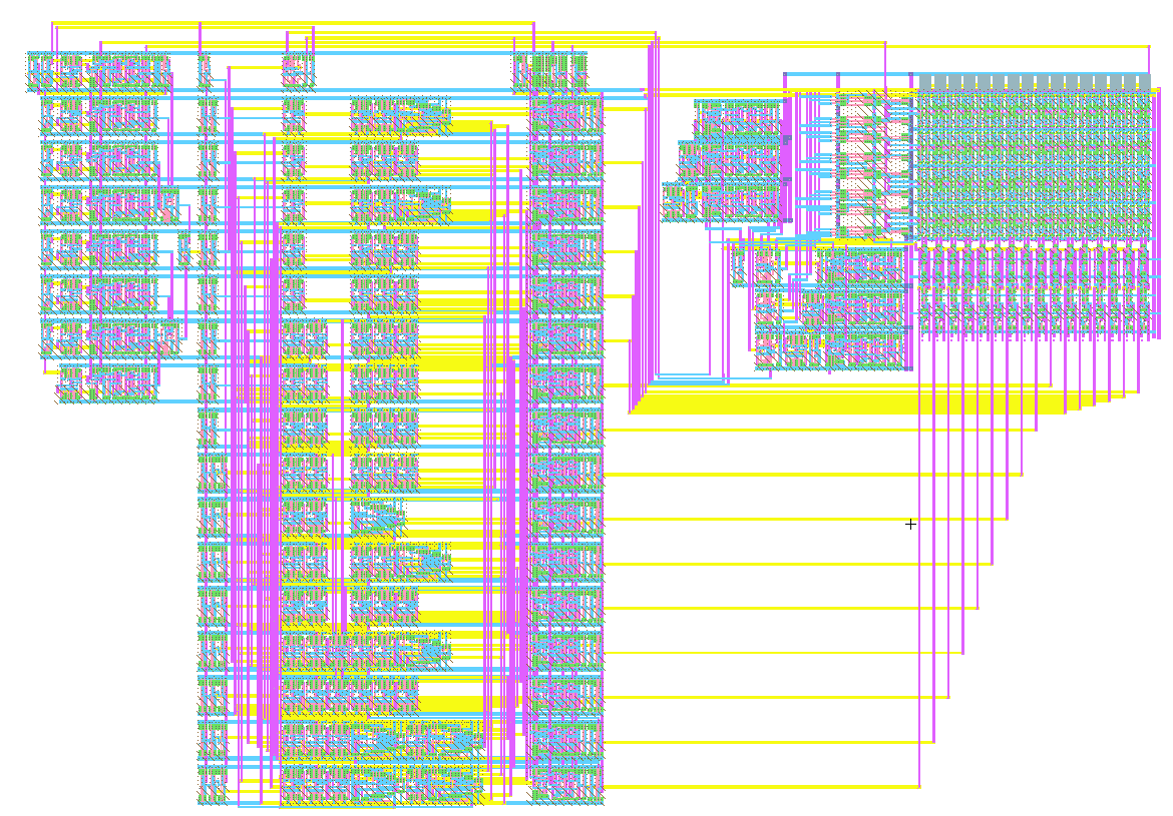
\includegraphics[width=0.5\textwidth]{layout1}
  \caption{Layout of the fingerprinting circuit with ALU and Memory fingerprinting using SRAM}
\end{figure}

% might be nice to add a block diagram of the circuit here%

\section{Experimental Setup and Verification}
The schematic and layout implementation of fingerprinting was done under Electric. However Electric is not able to verify functionality therefore Electric and IRSIM were used. This was achievable through exporting the schematic and layout information in Verilog deck.

\subsection{Schematic Verification}
Benchmarks were written in system verilog and simulated using ModelSim for functional verification. Each major circuit component was first simulated on the schematic level before implementing the layout. This not only aids in finding and fixing bugs, but also simplifies the component integration process. Random test vectors were generated to verify timing sequence and operation of complex circuits.

For the final circuit, the modified mips core was hooked up to the fingerprinting circuit for functional simulation. A benchmark was written in MIPS assembly to run on the mips core, and the produced waveform was studied to ensure proper circuit operation. 

\subsection{Layout Verification}
Our implemented circuit passes the DRC, ERC and NCC tests provided by Electric. Therefore all results obtained for the schematic of our circuit is valid for our layout design.


\subsection{Timing Analysis}
\subsubsection {\qquad  IRSIM}
Irsim, which is a“switch-level”digital circuit simulator, is used to perform a timing analysis for the fingerprint design. IRSIMl would generate a timing simulation based on the extracted capacitance and lumped resistance from the transistors in the circuit.
    
The Irsim simulation requires a Irsim deck, a prm file and a testbench file for simulation. The irsim deck, which contains all the connection information of the transistors in the schematic(or layout) design, can be automatically generated from Electric. A prm file, available from the Irsim Built-in lib, consists of all the resistance and capacitance value of transistors based on the technology involovd. The testbench can be written based on Irsim test-language-grammer.
    
The components of the fingerprinting design, including the multiplexer, the CRC circuit and the counter, are simulated individually for their path delay. This path delay can be found by observing the time difference between a rising clock edge and its next output value transition. Also, an average delay value from a set of distinct clocking edges is calculated to counter the value variance from different time intervals.

\subsubsection {\qquad  SRAM timing}
A 6T SRAM cell functions due to the 6 specially sized transistors that enable read and write stability. Since Modelsim is a functional/logic simulator which doesn’t consider transistor sizes, fifo cannot be tested in Modelsim with the rest of the circuit. Ideally, an SRAM cell model must be built which mimics the SRAM behaviour using logic. Since this would be time consuming, the entire circuit was instead tested with the earlier shift register implementation for functional verification. The fifo was also validatedl (IRSIM) which uses the linear delay model to approximate switching delay. 

The functionality was validated by observing internal signals in the FIFO block to verify each component behaved as intended with the right set of inputs. Once verified individually, two sets of tests were performed. The first test checked whether the FIFO can write 8 fingerprints in a row sequentially and read them out sequentially after some arbitrary time. The other test alternates write followed by a subsequent read. This test is more realistic considering fingerprints are generated one every few hundred/ thousand clock cycles. Once validated, the SRAM was connected to the entire circuit and a timing simulation was performed to evaluate the delay.

\section{Results}


\subsection{Area Overhead and Scaling}


\begin{center}
  \begin{tabular}{ l || c | r }
    \hline
     & Shift register & FIFO  \\ \hline
    Transistor count & 3872 & 1374 \\ \hline
    Area(lamda squared) & 2328 X 1000  & 1200 X 730 \\
    \hline
  \end{tabular}
\end{center}

The SRAM based design needs 3 times fewer transistors compared to the FF based design, consequently needing 3 times less area as shown in Figure 2. The area could have been smaller if the row decoder was built using a 45 lamda pitch, if the 3-bit counters were built using latches rather than the generic FFs and if the white space could have been eliminated by using a less modular design. The SRAM block and consequently the read and write drivers could have been tighter if there was an additional layer to route vdd and gnd wires.	

\begin{figure}[h!]
  \centering

      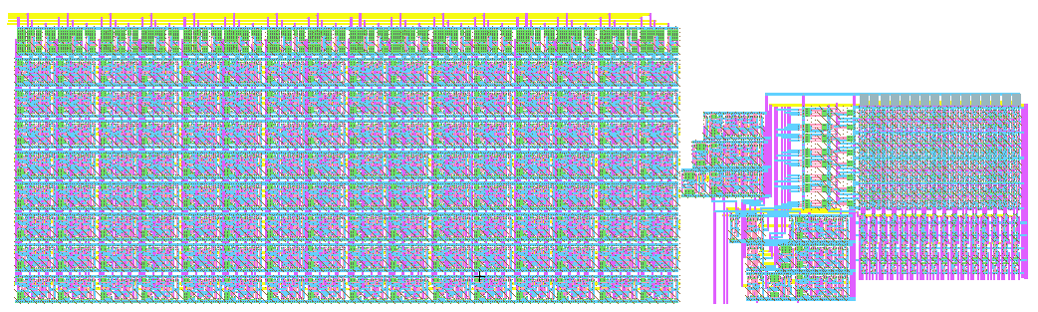
\includegraphics[width=0.5\textwidth]{layout}
  \caption{Layout comparison of FF design (left) and SRAM based (right)}
\end{figure}

% a note about how SRAM area compares to register area (even though it was mentioned already %
The fingerprinting circuit can be tuned for various modes of operation, and some decisions have an impact on area and cost. The counter determines the compression ratio, so increasing the counter's modulus will decrease the area required to store the fingerprints for the same amount of CPU execution information. Another important factor is the choice of execution data to fingerprint. At a minimum, the fingerprinting circuit needs to verify memory writes and adresses for data corruptions. However, if aditional data, such as ALU operations, are also fingerprinted, the amount of execution data will increase, and so will the area required to store all fingerprints. The impact of fingerprinting additional data would vary depending on the target application, but for the MIPS benchmark that we tested, the area required for storage gets tripled if ALU operations are fingerprinted in addition to memory write operations. 

\subsection{Operating Frequency}

 
As all the 16 bits in fingerprinting block are processed in parallel, each bit is simulated individually and differently for their single-bit path delay. The purpose of this test is to find the the slowest bit of the fingerprinting block. From the simulation, it is observed that the largest single-bit delay is 3.4ns, while the shortest is 2.27ns.

 From the simulation, it is shown that a reset signal from the counter will always slow down the CRC code output, due to the additional delay from the generation of these reset signals. Therefore, in order to find the worst case scenario of the system delay, only clock edges with a reset signal are analysed. From the collected data, the maximum delay for the design is found to be 6.90ns. To ensure the reliability of the worst case scenario, the range from “slowest bit” analysis mentioned above is also added to the worst case analysis. Table 1 shows the maximum delay of each component and of the system in order to determine the maximum operating frequency. The whole system delay is found to be 8.03ns. Based on this result, the maximum system operating frequency is estimated to be 125 Mhz. 
    
    \begin{table}[ht] 
\caption{Max Delay of Each Components and System} % title of Table 
\centering % used for centering table 
\begin{tabular}{c c c c c} % centered columns (4 columns) 
\hline\hline %inserts double horizontal lines 
Mux & Counter & Fingerprint & Shift Register & System\\ [0.5ex] % inserts table 
%heading 
\hline % inserts single horizontal line 
\\ [0.2 ex]
0.170ns & 0.990ns & 4.334ns & 0.892ns & 6.900ns \\ [1ex] % [1ex] adds vertical space 
\hline %inserts single line 
\end{tabular} 
\label{table:nonlin} % is used to refer this table in the text 
\end{table} 


\section{Conclusion}
One of the key observations from this project is the importance of understanding the limitations of tools used. For example, we learned after the project that NCC may not be reliable for large designs. So, while SRAM was tested for timing using the schematic description, the layout, though passing NCC, may be incorrect. Hence, if more time was available, the SRAM fifo layout would have also been thoroughly tested for any inconsistencies. Furthermore, the fifo could have been optimized further, for example by performing a path effort analysis for the row decoder. This would have shortened the time required to charge the capacitance of all the 16 SRAM cells and allowed for a higher operational frequency. 
The project would have benefited with more time evaluating the circuit in IRSIM because a timing analysis exposes various vulnerabilities of the design that Modelsim cannot check for. 

Wiring proved to be a challenge when implementing the layout. If the design was to be repeated, more attention would be placed on wire planning and pitch matching than on logic minimization, as a decrease in functional blocks or transistor count may not necessarily lead to improvements in area, and pitch matching can allow for menial tasks such as wire routing to be left to automation tools rather than the designer. Long and complex wires also decrease the modularity of a design, introduce additional parasitic resistances and capacitances, and make the system more vulnerable to noise, so it is generally a good idea to try and minimize them.

For this project, we have started with an early implementation of fingerprinting using only memory writes and storing in shift register. However, through better design iteration, we are now able to fingerprint ALU results and storing in SRAM which is much more efficient and provides better error detection capability.



\begin{thebibliography}{1}


\bibitem{DTR}
 Brett H. Meyer, Benton Calhoun, John Lach, Kevin Skadron, \emph{Cost-effective Safety and Fault Localization using Distributed Temporal Redundancy},CASES'11, October 2011.

\bibitem{RD}
Brett H. Meyer, Nishant George, Benton Calhoun, John Lach, Kevin Skadron, \emph{Reducing the Cost of Redundant Execution in Safety-Critical Systems using Relaxed Dedication}, DATE'11, March 2011.


\bibitem{harvey}
Havery Mudd College \emph{E158 Spring 2007 MIPS Project} [Online]. Available: http://www4.hmc.edu:8001/Engineering/158/07/project/index.html

\bibitem{electric}
Static Free Software, \emph{Electric} [Online]. Available: http://www.staticfreesoft.com/electric.html

\bibitem{techcon}
Mojing Liu, Jonah Caplan, Georgi Z. Kostadinov, and Brett H. Meyer, \emph{Workload Effects on Execution Fingerprinting for Low-cost Safety-Critical-Systems},  Semiconductor Research Corporation TECHCON 2013, September 2013.

\bibitem{Koopman}
P. ~Koopman and T.~Chakravarty, \emph{Cyclic Redundancy Code ({CRC}) Polynomial Selection For Embedded Networks}, Proceedings of the 2004 International Conference on Dependable Systems and Networks, 2004.

\bibitem{Parcrc}
E. ~Stavinov, \emph{A Practical Parallel {CRC} Generation Method}, Feature Article, pp. 38-45, Jan. 2010. 

\end{thebibliography}





%\vfill

% Can be used to pull up biographies so that the bottom of the last one
% is flush with the other column.
%\enlargethispage{-5in}



% that's all folks
\end{document}

